% !TEX TS-program = pdflatex
% !TEX encoding = UTF-8 Unicode

% This is a simple template for a LaTeX document using the "article" class.
% See "book", "report", "letter" for other types of document.

\documentclass[11pt]{article} % use larger type; default would be 10pt

\usepackage[utf8]{inputenc} % set input encoding (not needed with XeLaTeX)

%%% Examples of Article customizations
% These packages are optional, depending whether you want the features they provide.
% See the LaTeX Companion or other references for full information.

%%% PAGE DIMENSIONS
\usepackage{geometry} % to change the page dimensions
\geometry{a4paper} % or letterpaper (US) or a5paper or....
% \geometry{margin=2in} % for example, change the margins to 2 inches all round
% \geometry{landscape} % set up the page for landscape
%   read geometry.pdf for detailed page layout information

\usepackage{graphicx} % support the \includegraphics command and options

% \usepackage[parfill]{parskip} % Activate to begin paragraphs with an empty line rather than an indent

%%% PACKAGES
\usepackage{float} %used for figure placement with H as a parameter
\usepackage{booktabs} % for much better looking tables
\usepackage{array} % for better arrays (eg matrices) in maths
\usepackage{paralist} % very flexible & customisable lists (eg. enumerate/itemize, etc.)
\usepackage{verbatim} % adds environment for commenting out blocks of text & for better verbatim
\usepackage{subfig} % make it possible to include more than one captioned figure/table in a single float

\usepackage{multirow}
\usepackage{setspace}
% These packages are all incorporated in the memoir class to one degree or another...

%% Java Code Presentation
\usepackage{listings}
\usepackage{color}

\definecolor{dkgreen}{rgb}{0,0.6,0}
\definecolor{gray}{rgb}{0.5,0.5,0.5}
\definecolor{mauve}{rgb}{0.58,0,0.82}

\lstset{frame=tb,
  language=Java,
  aboveskip=3mm,
  belowskip=3mm,
  showstringspaces=false,
  columns=flexible,
  basicstyle={\small\ttfamily},
  numbers=none,
  numberstyle=\tiny\color{gray},
  keywordstyle=\color{blue},
  commentstyle=\color{dkgreen},
  stringstyle=\color{mauve},
  breaklines=true,
  breakatwhitespace=true,
  tabsize=3
}
%% End Java Code Presentation



%%% HEADERS & FOOTERS
\usepackage{fancyhdr} % This should be set AFTER setting up the page geometry
\pagestyle{fancy} % options: empty , plain , fancy
\renewcommand{\headrulewidth}{0pt} % customise the layout...
\lhead{}\chead{}\rhead{}
\lfoot{}\cfoot{\thepage}\rfoot{}

%%% SECTION TITLE APPEARANCE
\usepackage{sectsty}
%\allsectionsfont{\sffamily\mdseries\upshape} % (See the fntguide.pdf for font help)
\sectionfont{\normalfont\fontfamily{phv}\fontsize{16}{19}\bfseries}
\subsectionfont{\normalfont\fontfamily{phv}\fontsize{14}{17}\bfseries}
\subsubsectionfont{\normalfont\fontfamily{phv}\fontsize{14}{17}\selectfont}
% (This matches ConTeXt defaults)

%%% ToC (table of contents) APPEARANCE
\usepackage[nottoc,notlof,notlot]{tocbibind} % Put the bibliography in the ToC
\usepackage[titles,subfigure]{tocloft} % Alter the style of the Table of Contents
\renewcommand{\cftsecfont}{\rmfamily\mdseries\upshape}
\renewcommand{\cftsecpagefont}{\rmfamily\mdseries\upshape} % No bold!

%%% END Article customizations

%%% The "real" document content comes below...

\title{Brief Article}
\author{The Author}
%\date{} % Activate to display a given date or no date (if empty),
         % otherwise the current date is printed 

\begin{document}\newpage
\begin{center}
\thispagestyle{empty}
\Large{\textbf{A PROJECT REPORT\\ \large{ON}}}\\[0.7cm]
\LARGE{\textsc {\textbf{TRAVEL RESERVATION SERVICE}}}\\[0.5cm]
\vspace{0.5cm}
\Large{\textbf{\\Submitted to}}
\LARGE{\textbf{\\UNIVERSITY BORDEAUX 1\\}}
\vspace{1cm}
\vspace{1cm}
\Large{\textbf{\\BY}}\\[0.5cm]
\begin{table}[h]
\centering
\Large{
\begin{tabular}{>{\bfseries}lc>{\bfseries}l}
NGUYEN Quang Anh & & Team Leader\\
TRAN Thanh Phu & & Member\\
\end{tabular}}
\end{table}
\vspace{1.5cm}
\large{\textbf{MASTER INFORMATIC - SOFTWARE ENGINEERING}}\\
\Large{\textbf{UNIVERSITY BORDEAUX 1}}\\
\large{\textbf{\\2014-2015}}\\
\vspace{1cm}
\newpage
\end{center}
\newpage

%\newpage
\begin{center}
\thispagestyle{empty}
\Large{\textbf{A PROJECT REPORT\\ON}}\\[0.3cm]
\Large{\textsc {\textbf{``NAME OF PROJECT''}}}\\
\Large{\textbf{\\Submitted to}}
\LARGE{\textbf{\\UNIVERSITY OF PUNE\\}}
\large{\textbf{\\In Partial Fulfilment of the Requirement for the Award of\\}}
\LARGE{\textbf{\\BACHELOR'S DEGREE IN\\COMPUTER ENGINEERING}}
\vspace{0.3cm}
\Large{\textbf{\\BY}}\\[0.3cm]
\begin{table}[h]
\centering
\Large{
\begin{tabular}{>{\bfseries}lc>{\bfseries}r}
GROUP MEMBER A & & ROLL NUMBER A\\GROUP MEMBER B & & ROLL NUMBER B\\GROUP MEMBER C & & ROLL NUMBER C\\GROUP MEMBER D & & ROLL NUMBER D\\
\end{tabular}}
\end{table}
\large{\textbf{UNDER THE GUIDANCE OF}}\\
\large{\textbf{PROF. GUIDE NAME}}\\[0.5cm]

\includegraphics[scale=0.5]{project/images/jscoe_logo}\\
\large{\textbf{DEPARTMENT OF COMPUTER ENGINEERING}}\\
\Large{\textbf{NAME OF COLLEGE}}\\
\large{\textbf{LOCATION IN PUNE, PUNE - PINCODE}}
\large{\textbf{\\2012-2013}}\\[0.5cm]
\Large{\textbf{AFFILIATED TO}}\\[0.5cm]

\includegraphics[scale=5.0]{project/images/uop-logo}\\
\LARGE{\textbf{UNIVERSITY OF PUNE}}
\newpage

\end{center}
%\newpage

% includes the certificate page
%\begin{center}
\thispagestyle{empty}

\LARGE{\textbf{NAME OF COLLEGE}} \\ 
\large{\textbf{Department of Computer Engineering}}\\
\large{\textbf{LOCATION IN PUNE, Pune – PINCODE}}\\[0.5cm]


\includegraphics[scale=0.5]{project/images/jscoe_logo}\\[0.5cm]

{\Huge \textbf{CERTIFICATE}}\\[0.5cm]
\end{center}
\linespread{1.13}
\large{\centering{This is certify that the project entitled}\\[0.2cm]
\textbf{\Large{\centering{``NAME OF PROJECT``}}}\\[0.2cm]
\centering{submitted by}\\[0.2cm]
\begin{table}[h]
\centering
\large{
\begin{tabular}{>{\bfseries}lc>{\bfseries}r}
GROUP MEMBER A & & ROLL NUMBER A\\GROUP MEMBER B & & ROLL NUMBER B\\GROUP MEMBER C & & ROLL NUMBER C\\GROUP MEMBER D & & ROLL NUMBER D\\
\end{tabular}}
\end{table}
 is a record of bonafide work carried out by them, in the partial
 fulfilment of the requirement for the award of Degree of Bachelor of
 Engineering (Computer Engineering) at NAME OF COLLEGE, Pune under the 
 University of Pune. This work is done
 during year 2012-2013, under our guidance.}\\[0.5cm]
\large{\textbf{Date:\hspace*{1.0cm}/\hspace*{1.0cm}/}}\\
\begin{spacing}{0}
\vspace{3.0cm}
\large{\textbf{(Prof. GUIDE NAME)}}\hspace*{1.2in}\large{\textbf{(Prof. PROJECT COORD NAME)}}\\
\hspace*{0.7in}\textbf{Project Guide}\hspace*{2.3in}\textbf{Project Coordinator}\\[3cm]
\hspace*{0.5cm}\large{\textbf{(Prof. HOD NAME)}}\hspace*{0.8in}\large{\textbf{(Dr. PRINCIPAL NAME)}}\\
\textbf{HOD, Computer Department}\hspace*{0.8in}\textbf{Principal}\hspace*{1.1in}\textbf{External Examiner}
\end{spacing} 
%\newpage

% includes the acknowledgements page
%\begin{center}
\thispagestyle{empty}
\LARGE{\textbf{Acknowledgements}}\\[1cm]
\end{center}
\linespread{1.13}
\large{\paragraph{}We are profoundly grateful to \textbf{Prof. GUIDE NAME} for his expert guidance
and continuous encouragement throughout to see that this project rights its
target since its commencement to its completion.}
\large{\paragraph{}We would like to express deepest appreciation towards \textbf{Dr. PRINCIPAL NAME},
Principal, NAME OF COLLEGE, \textbf{Prof. HOD NAME}, 
Head of Department of Computer Engineering and \textbf{Prof. PROJECT COORDINATOR NAME}, Project Coordinator whose
invaluable guidance supported us in completing this project.}
\large{\paragraph{}At last we must express our sincere heartfelt gratitude to all the staff members
of Computer Engineering Department who helped me directly or indirectly during this course of work.}
\begin{flushright}
{
GROUP MEMBER A\\
GROUP MEMBER B\\
GROUP MEMBER C\\
GROUP MEMBER D
}
\end{flushright}
\newpage
 
%\newpage

\begin{center}
\thispagestyle{empty}
\vspace{2cm}
\LARGE{\textbf{ABSTRACT}}\\[1.0cm]
\end{center}
\thispagestyle{empty}
\large{\paragraph{}
Design pattern is a strong tool in Object Oriented Programming. The purpose of this project is to test the ability of understanding and implementing the design patterns. 
}
\large{\paragraph{}
In this project, I have implemented 11 design patterns. They are Singleton, Abstract Factory, Builder, Proxy, Composite, Decorator, Observer, Iterator, Visitor, Template
}\\ % adds the Research Methodology page
\newpage

%TABLE OF CONTENTS AND LIST OF FIGURES ARE AUTOMATICALLY ADDED BY FOLLOWING COMMANDS
%ADD FIGURE OF TABLES IF YOU NEED TO, CHECK DOCUMENTATION
\pagenumbering{roman} %numbering before main content starts


%To reset the Header & Footer for TOC and LOF
\pagestyle{empty}
\addtocontents{toc}{\protect\thispagestyle{empty}}
\doublespacing
\tableofcontents % adds Index Page
\singlespacing

\addtocontents{lof}{\protect\thispagestyle{empty}}
\listoffigures % adds List of Figures
\cleardoublepage

%And reset back the settings we choose for Header and Footer
\pagestyle{fancy}

\newpage
\pagenumbering{arabic} %reset numbering to normal for the main content

\section{INTRODUCTION}

\paragraph{}
In this project, we immitated a system that work for a travel agency. This system can book two main types of travel for the clients: travels without service and travels with services. Travel without service, means that the reservation is made only for the flight, where as travel with services allow a demand for checking in an hotel an renting a car.

\paragraph{}
For the purpose of simplify the input process, we prepared some input in advance. Below is the tables that present the flights available betweens the cities.

\paragraph{}
\begin{table}[h]
\centering
\begin{tabular}{|l|c|c|c|c|c|}
\hline
\multicolumn{1}{|c|}{\multirow{2}{*}{Departure}} & \multicolumn{5}{c|}{Destination} \\ \cline{2-6} 
\multicolumn{1}{|c|}{} & \multicolumn{1}{l|}{Paris} & \multicolumn{1}{l|}{Bordeaux} & \multicolumn{1}{l|}{Canberra} & \multicolumn{1}{l|}{Tokyo} & \multicolumn{1}{l|}{Delhi} \\ \hline
Hanoi & x & x & x & x & x \\ \hline
Hochiminh & x &  &  & x & x \\ \hline
Hue & x &  & x & x &  \\ \hline
Haiphong &  & x & x &  &  \\ \hline
Paris &  & x & x & x &  \\ \hline
Bordeaux & x &  &  & x & x \\ \hline
Canberra & x & x &  & x & x \\ \hline
Tokyo & x &  & x &  & x \\ \hline
Delhi & x &  & x & x &  \\ \hline
\end{tabular}
\end{table}

Between Hanoi, Hochiminh, Hue and Haiphong, there are flights between each other.  % adds the introduction page
\newpage

\section{PROGRAM 'S SPECIFICATION OVERVIEW}

\subsection{Brief Introduction}

\paragraph{}
Our project 's purpose is to help a travel agency make a booking for clients. There're two kinds of service package supported

\begin{itemize}
\item Travel without service: consist of only flight's reservation
\item Travel with services: apart from flight's reservation, hotel's reservation and car renting could also be added
\end{itemize}

\paragraph{}
There're three kinds of flight's reservation

\begin{lstlisting}
public enum FlightTicketType {
	VIP, Normal, Pool
}
\end{lstlisting}
The \textit{Pool} ticket is the type of ticket proposed to the travel agency by a flight agency. The only difference between \textit{Pool} and \textit{Normal} is that \textit{Pool}'s price is cheaper than the other.

\paragraph{}
There're also three kinds of hotel's reservation

\begin{lstlisting}
public enum HotelServiceType {
	Cheap, Normal, Lux
}
\end{lstlisting}

\subsection{Software Usage}

The creation of a Travel's object could be done using class \textit{TravelBuilder}. In this class, there're two methods that can create a travel without service

\begin{lstlisting}
public Travel buildTravelNoServiceForOneClient(Client c, FlightTicketType type, CityName destination)
public Travel buildTravelNoServiceForGroup(Client c, FlightTicketType type, CityName destination)
\end{lstlisting}

When a client register a service, if there isn't any direct flight between the client's current city and the destination city, a transit flight will be added.  

\paragraph{}
For creating a travel with services, consist of only one trip, we could use

\begin{lstlisting}
public Travel buildTravelSimpleService(Client c, CityName destination, FlightTicketType f, HotelServiceType h)
\end{lstlisting}

For a touring service, a trip through many cities, we need two functions

\begin{lstlisting}
public Travel buildTravelTouringService(Client c, CityName destination, FlightTicketType f, HotelServiceType h)
public void addNextTour(TravelTouringService t, CityName destination, FlightTicketType f, HotelServiceType h)
\end{lstlisting}

The first method is for building the first trip of the travel service. After that, anymore trip will be added using the second one. There's one problem in this setup, that's starting from the second trip, a trip to a new city must be a direct flight.




 
\newpage

\section{DESIGN PATTERNS}

\paragraph{}
In this project, I have used in total eleven design patterns. These patterns could be divided into three groups

\begin{itemize}
\item Creational: Singleton, Abstract Factory, Builder
\item Structural: Proxy, Composite, Decorator
\item Behavioral: Strategy, Observer, Iterator, Visitor, Template
\end{itemize}

\paragraph{}
The purpose of each pattern in this program will be presented briefly

\begin{itemize}

\end{itemize}
%\chapter{Requirement Analysis}
\section{SECTION NAME}
\paragraph{} WRITE HERE.
%\chapter{System Design}
\section{SECTION NAME}
\paragraph{} WRITE HERE.
%\chapter{System Testing}
\paragraph{} WRITE HERE.
\section{Test Cases and Test Results}
\begin{longtable}{ | p{1cm} | p{3.5cm} | p{4cm} | p{4cm} | p{4cm} |}
      \hline
      \textbf{Test ID} & \textbf{Test Case Title} & \textbf{Test Condition} & \textbf{System Behavior} & \textbf{Expected Result}\\
      \hline
      T01 & AAAA & BBBB & CCCC & DDDD\\
      \hline
      T02 & AAAA & BBBB & CCCC & DDDD\\
      \hline
      T03 & AAAA & BBBB & CCCC & DDDD\\
      \hline
\end{longtable}

\textbf{Note: Testing should be performed manually}
%\chapter{Project Planning}
\section{SECTION 1}
\paragraph{} WRITE HERE.

%\chapter{Implementation}
\paragraph{}WRITE HERE, PARAGRAPH 1.
\paragraph{}WRITE HERE, PARAGRAPH 2.

\begin{figure}[H]
  \centering
    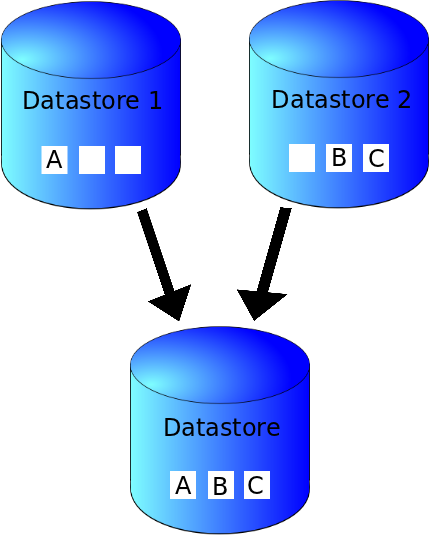
\includegraphics[scale=0.5]{project/images/data-sync}
  \caption{\textbf{IMAGE CAPTION}}
\end{figure}

\begin{lstlisting}
  PASTE YOUR CODE HERE
\end{lstlisting}
\newpage

 % adds the Project Design
%\chapter{Screenshots of Project}
\section{SECTION NAME}
\vspace{2cm}
\begin{figure}[H]
  \centering
    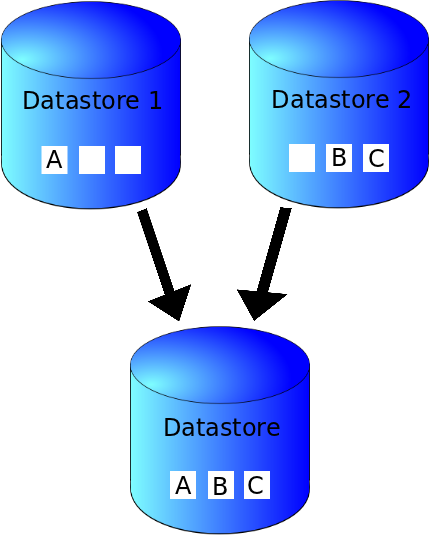
\includegraphics[height= 11cm, width=17cm]{project/images/data-sync}
\end{figure}
\newpage
\begin{figure}[H]
  \centering
    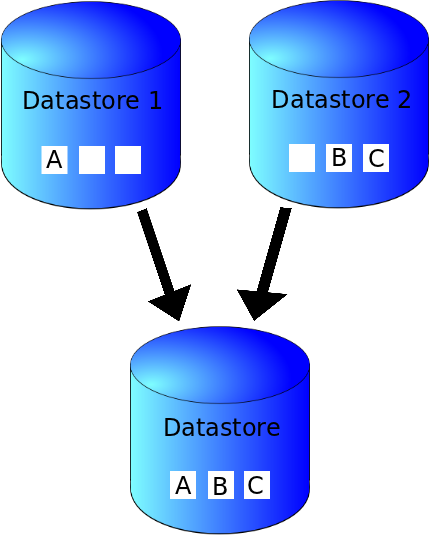
\includegraphics[height= 11cm, width=17cm]{project/images/data-sync}
\end{figure}
\vspace{1cm}
\begin{figure}[H]
  \centering
    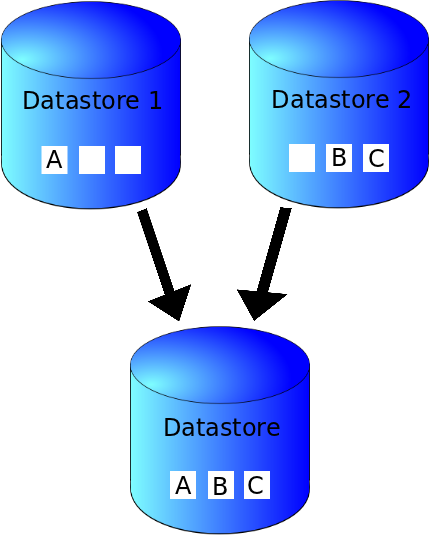
\includegraphics[height= 11cm, width=17cm]{project/images/data-sync}
\end{figure}
%\section{CONCLUSION}

\paragraph{}
After this project, I have obtained many knowledge, first of all, is the usage of many design patterns and the way to implement them. Secondly, I have learned about the flexibility when apply the design pattern, there are many way to implement a design pattern. You should choose a way that suit the situation the best rather than just mimicking the sample code. Lastly, I have learned the way to use Latex more efficiently in making a report % adds the Scheduling and Planning page
%\addcontentsline{toc}{chapter}{References}
\begin{thebibliography}{99}
\bibitem{WRITE A SHORT-NAME WITHOUT SPACE} \emph{NAME OF IEEE PAPER}; NAME OF AUTHORS
\bibitem{WRITE A SHORT-NAME WITHOUT SPACE} \url{http://EXAMPLE.com}
\end{thebibliography} % adds the References page

\end{document}
